\chapter{Survey study}
\label{ch:survey}
The second part of this research is to find out how we can determine the value ratios between TP, TN, FP, FN, and rejected predictions.
%
We conducted a literature study in section \ref{sec:related-work-value-assessment} and concluded that we want to empirically  estimate the value ratios from the perspective of the social media user.
%
In section \ref{sec:me}, we found that Magnitude Estimation (ME) seems like a promising technique for estimating these value ratios.
%
Therefore, this chapter discusses how we apply the ME technique in a crowdsourced survey study.
%

%
We design a survey study to ask participants the degree to which they agree or disagree with the decisions of a fictional social media platform called SocialNet.
%
We show the participants different scenarios representing TP, TN, FP, FN, and rejected predictions.
%
The TP and TN scenarios mean that SocialNet successfully detects whether a post is hateful or not, respectively.
%
The FP scenario means that SocialNet incorrectly predicts a non-hateful post as hateful, conversely for the FN scenario.
%
For example, in the FN scenario, the survey shows a hateful post to the participant and explains that SocialNet did not identify the post as hate speech.
%
Then, participants indicate the degree of agreement/disagreement using a scale, and we aggregate the answers per scenario to obtain the value ratios.
%

%
The structure and preparation of our crowdsourced survey study follow the pre-registration plan for social psychology suggested by \citet{van2016pre}.
%
In a pre-registration plan, we describe the hypothesis, procedure, and analysis before conducting the crowdsourced survey study to increase scientific credibility and reproducibility and reduce bias \citep{van2016pre}.
%
It is essential to select the statistical methods for the analysis part beforehand to prevent ourselves from selecting the statistic that best fits the collected data.
%
The content of this chapter reflects the final version of the pre-registration plan created after conducting the pilot survey.
%

%
In section \ref{sec:survey-hypothesis}, we make a hypothesis about the ME method and the value ratios.
%
Section \ref{sec:survey-method} contains all details about the setup of the survey.
%
Finally, in section \ref{sec:survey-analysis}, we elaborate on the analysis of the survey results.

\section{Hypothesis}
\label{sec:survey-hypothesis}
Before we conducted the survey experiment, we listed several hypotheses about the value ratios and the ME method:
\begin{itemize}
    \item \textbf{We hypothesize that the values of FP and FN are negative and that the value of an FN is lower than an FP}. We believe that both FP and FN predictions harm social media users; therefore, we think both values should be negative. We believe that allowing hateful content to be publicly visible has a more negative impact on social media users than filtering out neutral content. Therefore, we think an FN's value is lower than an FP's.
    \item \textbf{We hypothesize that the values of TP and TN are both positive and that the value of a TP is greater than a TN.} We believe that both TP and TN predictions positively impact social media users and, therefore, we think that both values should be positive. We believe predicting hateful content correctly is more valuable to social media users than correctly predicting non-hateful content. Therefore, we think a TP's value is greater than a TN's.
    \item \textbf{We hypothesize that the rejection value is negative and greater than the average value of an FP and an FN.} The critical assumption of using ML models with a reject option is that the negative value of rejection should always be greater than the negative value of an incorrect decision.
    \item \textbf{We hypothesize that Magnitude Estimation (ME) is a suitable technique for retrieving the value ratios.} ME seems like a promising technique for retrieving ratio data from judgements about hate speech detection scenarios. We use a 100-level numerical scale for validation. We expect that both scales are correlated and will give similar judgements. Although we also expect the 100-level scale to be suitable for retrieving opinions about the different hate speech detection scenarios, it does not provide the ratio data we need. We also expect that the inter-rater reliability for the 100-level scale will be higher than for the ME scale since the ME scale provides more response freedom. We also expect this since the authors of \citet{roitero2018fine} concluded that the inter-rater reliability of the 100-level scale is higher than the ME scale when rating the relevance of documents.
\end{itemize}

\section{Method}
\label{sec:survey-method}
In this section, we discuss the complete setup of the survey experiment and how we use both scales.

\subsection{Scales}
We use ME as the primary scale of our survey experiment.
%
As we concluded in section \ref{sec:me}, we must also validate the ME scale.
%
We validate the ME scale through cross-modality validation by comparing the results of the ME scale with another scale, as explained in section \ref{sec:me}.
%
The secondary scale is a bounded scale of 100 levels, called the 100-level scale, and we use this scale for four reasons.
%
First, given the limited budget, it is impractical in this project to use other ME scales, such as measuring the intensity of the participants' handgrips to express their judgements.
%
Second, there is no suitable dataset we can use for validation that contains human ratings of different scenarios in hate speech detection.
%
Third, we concluded in \ref{sec:likert} that Likert scales have limited response freedom.
%
Finally, in \citet{roitero2018fine}, the authors concluded that the 100-level scale provides more response freedom than course-grained Likert scales and has several advantages over ME in terms of usability and reliability.
%
The 100-level scale is easier to understand than ME, does not require normalization, and provides more flexibility than Likert scales \citep{roitero2018fine}.
%
Therefore, we will create two separate surveys with the same scenarios where half of all participants use the 100-level scale and the other half use the ME scale.
%
Both scales are bipolar scales since the participants should be able to either disagree or agree with the scenarios.

\subsection{Normalization}
The ME scale is unbounded and, therefore, provides a lot of response freedom.
%
For example, suppose we first show a scenario and the participant provides a value (e.g., 100) to indicate the degree of agreement.
%
Suppose we next present a scenario that the participant agrees with more.
%
The participant can always provide a higher value (e.g., 125).
%
However, the results need to be normalized as different participants rate the agreement/disagreement degree differently.
%
As explained in section \ref{sec:me}, we cannot use standard normalization methods such as geometric averaging as we use bipolar scales with negative values.
%
Therefore, we normalize the results by dividing the magnitude estimates of each participant by their maximum estimate.
%
We multiply the normalized magnitude estimates by 100 for the sake of clarity.
%
This way, all magnitudes estimates are in the range $[-100, 100]$ while maintaining the ratio properties.

\subsection{Design}
We will list all independent, dependent, confounding, and control variables analyzed in our experiment in this section.

\subsubsection{Independent variables}
Independent variables are the different hate speech detection scenarios we show to the participants (TP, TN, FP, FN, and rejection).
%
We inform the participants in the case of TP and FP scenarios that SocialNet ranks the hateful post lower on their feed.
%
The users then need to spend more effort finding the post since they need to scroll longer before it becomes visible.
%
We decided to explain that the hateful posts are ranked lower since we found significant disagreement among participants after the pilot survey in which we explained that SocialNet removes hateful posts.
%
We inform participants in the rejection scenarios that a human moderator needs to check the post (that can be either hateful or not hateful) within 24 hours.
%
Meanwhile, the post remains visible with its original rank on the user's feed.
%
We use 24 hours based on the German NetzDG law, which allows the government to fine social media platforms if they do not remove illegal hate speech within 24 hours \citep{tworek2019analysis}.
%
\begin{itemize}
    \item \textbf{True Positive} Show a hateful post to the user and explain that SocialNet detected hate and ranked the post lower on people's feeds.
    \item \textbf{True Negative} Show a non-hateful post to the user and explain that SocialNet did not detect hate and allowed the post.
    \item \textbf{False Positive} Show a non-hateful post to the user and explain that SocialNet detected hate and ranked the post lower on people's feeds.
    \item \textbf{False Negative} Show a hateful post to the users and explain that SocialNet did not detect hate and allowed the post.
    \item \textbf{Rejection}
          \begin{itemize}
              \item Show a hateful post to the user and explain that SocialNet was uncertain whether the post was hateful or not. An internal moderator will need to check the post within 24 hours. Meanwhile, the post remains visible.
              \item Or show a non-hateful post to the user and explain that SocialNet was uncertain whether the post was hateful or not. An internal moderator will need to check the post within 24 hours. Meanwhile, the post remains visible.
          \end{itemize}
\end{itemize}

\subsubsection{Confounding variables}
%
Confounding variables are the different demographic characteristics:
%
\begin{itemize}
    \item \textbf{Nationality} People from different nationalities might have different perceptions and definitions of hate speech and how we should deal with it.
    \item \textbf{Age} People of different ages might have different perceptions and definitions of hate speech and how we should deal with it.
    \item \textbf{Educational level} People with different educational levels might have different perceptions and definitions of hate speech and how we should deal with it.
    \item \textbf{Gender} According to \citet{gold2018women}, there is no significant difference in how men and women perceive hate. However, we still report gender as a confounding variable since we want to analyze if there are genuinely not any differences.
\end{itemize}

\subsubsection{Control variables}
%
We define two control variables: the measurement scales and the content of the social media posts we show to the participants.
%
We control the measurement scale variable by randomly assigning a participant to use either the 100-level or the ME scale to rate the scenarios.
%
Regarding the scales, as described before, we choose Magnitude Estimation as our primary scale and use the 100-level scale for validation.
%
We leave the study of other scales to future work.
%
We control the content of the social media posts in two manners.
%
First, we present all scenarios for all participants randomly to reduce bias.
%
Second, we sample the social media posts for the survey from existing datasets.
% 
We explain the selection procedure in section \ref{sec:data}.
%
\begin{itemize}
    \item \textbf{Scales} The first group of participants must answer the questions using the ME scale. The second group needs to answer the questions using the 100-level scale.
    \item \textbf{Content of the posts} We sample all social media posts from existing datasets and present them to the participants in random order.
\end{itemize}

\subsubsection{Dependent variables}
Our dependent variables are the response values, reliability, validity and the value ratio of TP, TN, FP, FN, and rejection scenarios.
%
\begin{itemize}
    \item \textbf{Response values} All response values the participants give to the different scenarios with either the ME or the 100-level scale.
    \item \textbf{Reliability} Measured using Krippendorff's alpha, where values larger than 0.8 indicate reliable conclusions and values larger than 0.6 indicate tentative conclusions \citep{krippendorff2004reliability}.
    \item \textbf{Validity} Convergent validity, if two different measures measure the same thing \citep{fitzner2007reliability}. Measured by calculating the correlation between the magnitude estimates and the response values from the 100-level scale.
    \item \textbf{Value ratios of TP, TN, FP, FN, and rejection scenarios} Measured by calculating the median of the normalized magnitude estimate response values of each scenario question and then calculating the mean over the resulting values to come up with the final value for that scenario type.
\end{itemize}

\subsection{Planned sample}
This section discusses how we pick the sample size, recruit the participants, and explains which stopping and exclusion rules we apply.

\subsubsection{Sample size}
There are 4.55 billion active social media users\footnote{\url{https://datareportal.com/reports/digital-2021-october-global-statshot}}.
%
We choose a 90\% Confidence Interval (CI) and 10\% Margin of Error (MoE) for this study.
%
So for 90\% of the time, our observations will fall within a 10\% interval \citep{olson2014ways}.
%
According to \citet{olson2014ways}, we need a sample size of 68 participants per survey type to reach the desired CI and MoE values.
%
We choose 10\% MoE since we have a limiting budget.
%
We first conduct a pilot survey for 12 participants per scale to gather feedback and check if we need to improve things before the actual experiment.
%
We want to determine the average workload using the pilot survey and decide whether reducing the MoE by increasing the number of participants is possible.
%
For the pilot survey, we use 24 participants.
%
Therefore, in total we will need $2*12+2*68 = 160$ participants.
%
Of the recruited participants, 50\% identified as female.
%
Half of the participants are assigned the ME scale, and the other half the 100-level scale.

\subsubsection{Participants}
We will use the \href{https://prolific.co}{Prolific} platform for recruiting online participants for the survey study.
%
We will use the following inclusion criteria for our participants:
\begin{itemize}
    \item 18 years of age and older since we show offensive language in the experiment.
    \item Fluent in English.
    \item Approval rating over 90\% on the Prolific platform.
    \item Use one of the following social media platforms regularly (at least once a month): Facebook, Twitter, YouTube, LinkedIn, Pinterest, Google Plus, Tumblr, Instagram, Reddit, VK, Flickr, Vine.co, Meetup, ask.fm, Snapchat, TikTok, Medium.
\end{itemize}
%
Every participant will be paid based on the hourly wage of 9.0 GBP (about 10,67 Euro), indicated as good pay by the platform\footnote{\url{https://prolific.co/pricing}}.
%
We use the following exclusion/rejection criteria:
\begin{itemize}
    \item Participants who fail the two attention checks. We will include two Instructional Manipulation Checks to check if the user pays attention to the survey\footnote{\url{https://researcher-help.prolific.co/hc/en-gb/articles/360009223553}}.
    \item Participants who do not complete all questions.
    \item Participants who disagree with the informed consent before the start of the survey. We are not allowed to collect and process their data if they do not consent.
    \item Participants who do fail the ME training phase. For example, by providing random values that do not make any sense.
\end{itemize}
%
We select a balanced set of participants in Prolific, among which 50\% are men and 50\% are women.

\subsection{Data}
\label{sec:data}
Depending on the assigned survey group, all subjects must judge several TP, TN, FP, FN, and rejection scenarios using either the ME or the 100-level scale.
%
We select the posts used in the scenarios from a public dataset \citep{basile2019semeval} that contains 13,000 English tweets.
%
Each tweet is annotated with three categories: hate speech (yes/no), target (generic group or an individual), and aggressiveness (yes/no).
%
Therefore, we have one neutral and four groups of hateful tweets: generic target + aggressive, individual target + aggressive, generic target + non-aggressive, and individual target + aggressive.
%
For the rejection scenarios, we need both neutral and hateful tweets.
%
Therefore, we need at least eight tweets per scenario type (TP, TN, FP, FN, and rejection).
%
We need 40 tweets, where 20 are hateful and 20 are not hateful, to create 40 different scenarios.
%
We want to select the most representative tweets from the dataset.
%
Randomly selecting the tweets from the dataset is insufficient as the dataset might contain sample retrieval bias, as explained in section \ref{sec:related-work-challenges}.
%
We might retrieve too many similar tweets about the same topic when randomly selecting the tweets.
%
Therefore, we perform content analysis to create a selection of tweets that is as representative and diverse as possible.
%
We provide an overview of our selection process in figure \ref{fig:clustering}.
%
We exclude all tweets that contain Twitter replies and mentions since  they have unclear contexts.
%
Then we preprocess all tweets by removing the URLs and hashtags.
%
Finally, we use clustering analysis to select 40 tweets for our study.
%
We perform latent semantic analysis (LSA) and k-means clustering on each group of tweets.
%
We use term frequency-inverse document frequency (TF-IDF) to represent all documents and their words, also known as terms, in a matrix where the term frequencies indicate how important that term is to the document \citep{aggarwal2012survey}.
%
The term frequencies are multiplied with the inverse document frequency so that terms that often occur in all documents, such as stop words, will end up with a lower value in the matrix \citep{aggarwal2012survey}.
%
Then, we use singular value decomposition (SVD) for dimensionality reduction to transform the output matrix of the TF-IDF step.
%
The transformed matrix is more suitable for text clustering techniques since documents with similar terms are now grouped \citep{aggarwal2012survey}.
%
The combination of TF-IDF and SVD is also known as LSA and is suitable for clustering purposes \citep{aggarwal2012survey}.
%
Finally, we apply the unsupervised learning technique k-means to the output of the LSA method to cluster all tweets into k clusters.
%
We calculate the silhouette coefficient to determine the optimal cluster size (k value) for the neutral tweets and the four groups of hateful tweets.
%
The silhouette analysis indicates to set k as large as possible.
%
We select the five nearest data samples to each cluster centroid.
%
From this selection, we manually choose one tweet per cluster using a majority vote from three group members to create the final set of 40 tweets.
%
Based on the silhouette coefficient, we use a cluster size of 20 for the neutral tweets and select one tweet per cluster to collect 20 neutral tweets.
%
Furthermore, we use a cluster size of 5 for each group of hateful tweets to collect 20 hateful tweets.
%
\begin{figure}
    \centering
    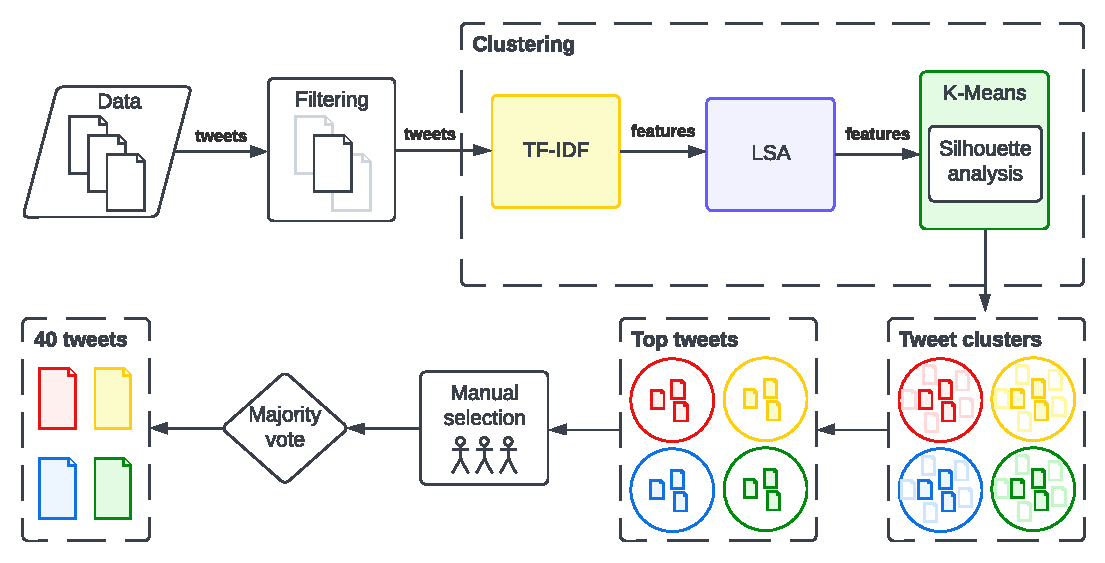
\includegraphics[width=\textwidth]{Figures/clustering.pdf}
    \caption{Flow diagram that visualizes how we perform content analysis to cluster and select the tweets for our survey study.}
    \label{fig:clustering}
\end{figure}

\subsection{Procedure}
We use LimeSurvey\footnote{\url{https://www.limesurvey.org/}} as our survey tool.
%
The survey first presents the informed consent policy and excludes participants that do not agree with it.
%
Next, we show introductory texts to the participants to explain what we will expect from them and to explain the structure of the survey.
%
Using the ME scale, we first present a warm-up task where the participants need to estimate different line lengths to get familiar with using the ME scale.
%
Then, we randomly present 40 scenarios representing the TP, TN, FP, FN, and rejection scenarios (with eight scenarios per type).
%
Each scenario contains several questions with the same structure.
%
The first question is whether participants think the post is hateful (yes/no).
%
The second question is whether participants agree, disagree, or are neutral with SocialNet's decision.
%
In the case of nonneutral, we ask a third question about the degree to which participants agree or disagree with the machine's decisions, using either the ME or 100-level scale, depending on their group.
%
There is no time limit for answering the questions, and all data is anonymous.
%
Finally, we will inform the participants not to put identifiers in their answers.
%
Refer to \autoref{sec:appendix} for all presentation texts, the informed consent, and some scenario examples.

\noindent\customtextbox{
    \begin{itemize}[leftmargin=*, label={}]
        \item \textbf{Step 1: provide informed consent}
              \begin{itemize}
                  \item Show the informed consent (with checkboxes for giving consent).
                  \item Proceed to the next step only for the participants who give consent.
              \end{itemize}
        \item \textbf{Step 2: introduction}
              \begin{itemize}
                  \item Show introductory text about what is expected from the participant.
                  \item We split all participants up into two groups.
                  \item The first group first uses the ME scale to rate all scenarios.
                  \item The second group first uses the 100-level scale to rate all scenarios.
                  \item Explanation of the scale.
              \end{itemize}
        \item \textbf{Step 3: two attention checks}
              \begin{itemize}
                  \item Two simple attention checks where we ask the participant to select one option (shuffled through all scenarios).
              \end{itemize}
        \item \textbf{Step 4a: ME practice phase (when ME is used)}
              \begin{itemize}
                  \item To let participants learn how to use ME, we first run a practice phase where we shuffle and present 5 different line lengths.
                  \item Each participant needs to estimate the line length using any positive value.
              \end{itemize}
        \item \textbf{Step 4b: all scenarios using the scale (ME or 100-level)}
              \begin{itemize}
                  \item Show 40 different scenarios in random order: 8 TP, 8 TN, 8 FP, 8 FN, and 8 rejection.
              \end{itemize}
        \item \textbf{Step 5: finish}
              \begin{itemize}
                  \item Show a thank you message and redirect the users to Prolific to complete the task.
              \end{itemize}
    \end{itemize}
}

\section{Analysis}
\label{sec:survey-analysis}
First, we calculate the value ratios of the TP, TN, FP, FN, and rejection scenarios in hate speech detection using the survey's results.
%
Second, we analyze the quality of our survey method by looking at two aspects: reliability and validity.

\subsection{Value ratios}
\label{sec:analysis-values}
The survey study aims to determine value ratios of the TP, TN, FP, FN, and rejection scenarios in the context of hate speech detection.
%
The metric from section \ref{sec:value-metric} takes these numerical values as input to calculate the optimal rejection threshold.
%
We do not need to know the absolute values but only the relative values.
%
For example, if we set all values to 1, we retrieve the same optimal rejection threshold as setting all values to 1000.
%
We use a bipolar scale for question 3 in the survey since we ask the participants the degree to which they agree, disagree, or are neutral with the decision of SocialNet.
%
For both scales, we will convert disagreement values to negative values, neutral values to 0, and agreement values to positive values.
%
Since we found that the data of both scales is skewed after conducting the pilot survey, we first apply the median to the individual questions' results.
%
Then we calculate the mean value over the resulting values to retrieve the final aggregated value ratios.
%
For example, to calculate the aggregated $V_{tp}$ values for both scales, we use:
\begin{align*}
    V_{tp}^{ME} = \frac{1}{n} \sum_{i=1}^{n} r_{i, tp}^{ME}   & \quad  \parbox{35em}{\footnotesize where $n$ is the total number of all participants for TP scenarios and $r_{i, tp}^{ME}$ is the  \\median response value of TP question number $i$ rated with the ME scale.}\\
    V_{tp}^{100} = \frac{1}{n} \sum_{i=1}^{n} r_{i, tp}^{100} & \quad  \parbox{35em}{\footnotesize where $n$ is the total number of all participants for TP scenarios and $r_{i, tp}^{100}$ is the \\median response value of TP question number $i$ rated with the 100-level scale.}
\end{align*}
%
We apply the same calculations for the remaining scenario types.
%
The results should give us an understanding of how the participants feel towards the different scenarios: TP, TN, FP, FP, and rejection.
%
We define the value ratios we need for the metric using the aggregated values of the TP, TN, FP, FN, and rejection scenarios rated with the ME scale since the ME scale provides us with ratio data.
%
We will not use the aggregated values of the 100-level scale for our metric since the 100-level scale does not provide ratio data, but we will still present them.

\subsection{Reliability}
Reliability is about whether we can trust our results and if we get consistent results \citep{fitzner2007reliability}.
%
We do this by mainly looking at the inter-rater reliability.
%
Different participants should give approximately the same judgements to the same scenarios.
%
We measure the inter-rater reliability using Krippendorff's alpha \citep{maddalena2017crowdsourcing, krippendorff2004reliability}.
%
We calculate the inter-rater reliability value for the complete survey's data for the normalized ME and 100-level values.
%
We use the inter-rater reliability scores to compare the ME scale with the 100-level scale.
%
We also separately study the inter-rater reliability values for the different types of scenarios (TP, TN, FN, FP, and rejection).
%
This experiment does not consider other types of reliability, such as test-retest reliability.
%
Guaranteeing test-retest reliability would require us to redo the complete experiment at a different time for the same participants, which is infeasible for this project, given the limited time and budget.

\subsection{Validity}
\label{sec:analysis-validity}
Validity is about whether we are measuring the things we want to measure \citep{fitzner2007reliability}.
%
The main goal of this aspect is to validate if we can use the ME technique to measure participants' opinions about hate speech detection scenarios.
%
There are multiple types of validity, but we focus mainly on convergent validity (part of construct validity), content validity, and face validity \citep{fitzner2007reliability}.
%
Construct validity checks whether there is an agreement between a theory and a measurement device or procedure \citep{fitzner2007reliability}.
%
Convergent validity is about the correlation between different measures to see if they measure the same phenomenon \citep{fitzner2007reliability}.
%
Content validity is about letting experts review the proposed research questions and procedure \citep{fitzner2007reliability}.
%
Face validity is a subjective type of validity, and it is about why we think the questions and proposed procedures are valid \citep{fitzner2007reliability}.
%

%
We analyze convergent validity by performing cross-modality validation.
%
Following the approach from \citet{roitero2018fine}, we analyze the correlation between the ME scale and the 100-level scale.
%
We can verify that they measure the same phenomenon if we find that both scales are positively correlated.
%
However, we can also expect a low correlation since the ME scale is a (normalized) unbounded scale and the 100-level scale is bounded.
%
Nevertheless, we think both scales will give similar results, meaning that high ME responses should correspond to high 100-level scale responses and low ME responses to low 100-level scale responses.
%
To guarantee content validity, we let experts (the supervisors of this thesis project) check the pre-registration report before conducting the experiments.
%
We tackled face validity in section \ref{sec:related-work-value-assessment} by arguing why we think the ME technique is suitable for measuring people's opinions about hate speech detection scenarios.
%
We exclude other forms of validity from this experiment because they are irrelevant or infeasible.
%
For example, external validity is about the degree to which the findings can be generalized to other settings or groups \citep{fitzner2007reliability}.
%
We think people with different demographic characteristics perceive hate speech differently since people have other norms and values.
%
We believe that if we conduct this experiment using different groups of participants, we might retrieve different value ratios.
%
Therefore, we decided not to create too many participant inclusion criteria but take a random sample of global social media users.
%
We would have to experiment with multiple groups with different demographic characteristics to guarantee external validity.
%
We left this for future work to investigate in full detail.
%
However, we still try to analyze if we can find any differences between participants with different demographic characteristics in the dataset we retrieve (refer to section \ref{sec:analysis-demographic}).

\subsection{Demographics}
\label{sec:analysis-demographic}
As we conduct the survey study only once for a group of participants, among which 50\% are men and 50\% are women, the remaining demographic characteristics can be quite diverse.
%
Nevertheless, we are still curious if there are any significant statistical differences between groups of participants with different demographic characteristics as we expect that demographic characteristics influence people's perception of hate speech and how we should deal with it.
%
Therefore, we apply several statistics to the results of each scenario to analyze if we can find differences between different demographic groups.
%
Prolific provides information about the demographic characteristics of the participants, out of which we analyze four variables: nationality, age, student (whether they are still a student or not), and gender.
%
We have multiple groups (more than two) for the variables nationality and age (different age intervals) and two groups for the variables student and gender.
%
We apply either analysis of variance (ANOVA) (parametric) or Kruskal-Wallis (non-parametric) when we have more than two groups and apply an unpaired two-samples t-test (parametric) or the Mann-Whitney U Test (non-parametric) when we have exactly two groups.
%
First, we check if we can apply the parametric statistics by checking if their assumptions hold in our dataset.
%
If not, then we use the non-parametric tests.
%
We apply ANOVA and the t-test when the data meets the following three conditions: homogeneity of variance (each population has the same variance), normality (normal distribution of the error), and independence (the observations are independent of each other) \citep{howell2012statistical}.
%
We use Bartlett's test of homogeneity of variances and the Shapiro-Wilk test of normality to check if we can apply ANOVA and the t-test.
%
We obey the independence condition since we collect the data of all participants of our survey study Independently.
%
ANOVA and the t-test can be robust to violations of the homogeneity of variances and the normality assumptions \citep{howell2012statistical}.
%
However, if one of the assumptions is violated then it is important to keep the sample sizes as equal as possible \citep{howell2012statistical}.
%
\todo[inline]{explain pairwise analysis. We use pairwise parametric tests (t-test) or pairwise non-parametric tets (mann-whitney u test) to test if there any differences between the different groups when ANOVA or Kruskal-Wallis is used. However, is this results into many extra statistical tests, there is a chance of introducting Type I errors, meaning that we incorrectly reject the null hypothesis for some of the tests. This would indicate that we find significant differences between the groups while there aren't any. Therefore, we perform the post-hoc Benjamini-Hochberg procedure for correcting the p-values to control the Type I errors.}